\subsection{Union, Intersection, Difference, and Complement}

\begin{definition} \label{def:analysis-sets-and-operations} \hlt{Elementary Set Operations}\\
Let $X$ be a set and let $A,B\subseteq X$.
\begin{enumerate}[label=(\roman*)]
\setlength{\itemsep}{0pt}
\item \hlt{Union}: $A\cup B\defeq\{x\in X:x\in A\text{ or }x\in B\}$.
\item \hlt{Intersection}: $A\cap B\defeq\{x\in X:x\in A\text{ and }x\in B\}$.
\item \hlt{Difference}: $A\setminus B\defeq\{x\in X:x\in A\text{ and }x\notin B\}$.
\item \hlt{Complement}: $A^c\defeq X\setminus A$, relative to the ambient set $X$.
\end{enumerate}
\end{definition}

\begin{definition} \label{def:symmetric-difference-of-events-and-sets} \hlt{Symmetric Difference}\\
Let $X$ be a set and let $A,B\subseteq X$.
The \hlt{symmetric difference} is $A\triangle B\defeq(A\setminus B)\cup(B\setminus A)$.\\
It consists exactly of the elements belonging to one of $A$ and $B$, but not both.
\end{definition}

\begin{proposition} \label{prop:analysis-set-algebra} \hlt{Basic Set Algebra}\\
Let $X$ be a set and let $A,B,C\subseteq X$. Then
\begin{enumerate}[label=(\roman*)]
\setlength{\itemsep}{0pt}
\item $A\cap(B\cup C)=(A\cap B)\cup(A\cap C)$;
\item $A\cup(B\cap C)=(A\cup B)\cap(A\cup C)$;
\item $(A\cup B)^c=A^c\cap B^c$;
\item $(A\cap B)^c=A^c\cup B^c$;
\item $A\triangle B=(A\cup B)\setminus(A\cap B)$.
\end{enumerate}
\begin{proof}
Fix an arbitrary $x\in X$.
By set extensionality, each identity follows once its two membership conditions are equivalent.
\begin{enumerate}[label=(\roman*)]
\setlength{\itemsep}{0pt}
\item[(i)] Membership in $A\cap(B\cup C)$ means that $x\in A$ and that either $x\in B$ or $x\in C$.
This holds exactly when either $x\in A\cap B$ or $x\in A\cap C$.
Hence it is equivalent to membership in $(A\cap B)\cup(A\cap C)$.
\item[(ii)] Membership in $A\cup(B\cap C)$ means that $x\in A$, or that both $x\in B$ and $x\in C$.
This holds exactly when two conditions are satisfied.
First, $x\in A$ or $x\in B$; second, $x\in A$ or $x\in C$.
Hence it is equivalent to membership in $(A\cup B)\cap(A\cup C)$.
\item[(iii)] The condition $x\in(A\cup B)^c$ is equivalent to $x\notin A\cup B$.
This means that $x\notin A$ and $x\notin B$, or equivalently $x\in A^c\cap B^c$.
\item[(iv)] The condition $x\in(A\cap B)^c$ is equivalent to $x\notin A\cap B$.
This means that $x\notin A$ or $x\notin B$, or equivalently $x\in A^c\cup B^c$.
\item[(v)] The condition $x\in A\triangle B$ is equivalent to $x\in A\setminus B$ or $x\in B\setminus A$.
Thus $x$ belongs to one of $A$ and $B$, but not both.
Equivalently, $x\in A\cup B$ and $x\notin A\cap B$.
By the definition of difference, this is equivalent to $x\in(A\cup B)\setminus(A\cap B)$.
\end{enumerate}
\hlt{Structural Commentary}: Each identity reduces to an equivalence of membership conditions.\\
\hlt{Key Insight}: Membership turns set operations into logical connectives.\\
\end{proof}
\end{proposition}

\begin{illustrationfigure}[H]
    \centering
    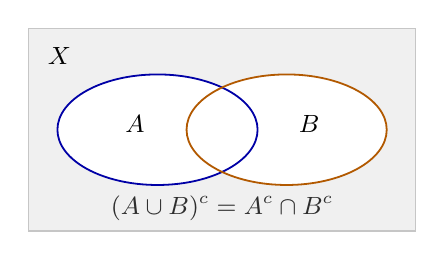
\begin{tikzpicture}[
  x=0.82cm,
  y=0.78cm,
  every node/.style={font=\small},
  ambient/.style={draw=gray!45, fill=gray!12, line width=0.5pt},
  setA/.style={draw=blue!65!black, line width=0.65pt},
  setB/.style={draw=orange!70!black, line width=0.65pt}
]
  \draw[ambient] (-3,-1.65) rectangle (3,1.65);
  \fill[white] (-1.0,0) ellipse (1.55 and 0.9);
  \fill[white] (1.0,0) ellipse (1.55 and 0.9);
  \draw[setA] (-1.0,0) ellipse (1.55 and 0.9);
  \draw[setB] (1.0,0) ellipse (1.55 and 0.9);

  \node at (-1.35,0.1) {$A$};
  \node at (1.35,0.1) {$B$};
  \node[anchor=north west] at (-2.85,1.5) {$X$};
  \node[gray!35!black] at (0,-1.28) {$(A\cup B)^c=A^c\cap B^c$};
\end{tikzpicture}

    \caption{The shaded region represents $(A\cup B)^c=A^c\cap B^c$ inside the ambient set $X$.}
    \label{fig:de-morgan-complement-union}
\end{illustrationfigure}

Figure \ref{fig:de-morgan-complement-union} illustrates part (iii).
The shaded region lies outside both $A$ and $B$, so it is outside $A\cup B$.
